\section{Closed-Loop Simulation and Ablations}\label{sec:sim}
\textbf{Why a simulator.} Hardware runs are slow and uncontrolled. We built a
closed-loop plant in which CPU utilisation of the chosen rung heats a
first-order thermal mass (optionally with a second slow mass, temperature-dependent
leakage and ambient steps), firmware throttling cuts speed and heat, and
policies drive the \emph{real} decision engine in virtual time. Rung operating
points and the throttle penalty are \textbf{assumptions}; every simulated number
carries the mark~\SIM{} and none is evidence about a device until the plant is
fitted (E7, Table~\ref{tab:fidelity}; fit $R^2=$ \resPlantR).

\begin{table*}[t]
\centering\small
\caption{Simulated policy comparison (assumed plant, 10 seeds).}\label{tab:sim}
\begin{tabular}{lrrrrr}
\toprule
Scenario & Policy & Utility & p5 & $>$70\,\textdegree C \% & Sw/h \\
\midrule
cool-room & static-0 & 7.43$\pm$0.56 & 5.48$\pm$1.74 & 96$\pm$1 & 0$\pm$0 \\
cool-room & thermostat & 6.42$\pm$0.95 & 4.39$\pm$1.96 & 58$\pm$20 & 60$\pm$38 \\
cool-room & shade-noguards & 5.81$\pm$0.68 & 4.00$\pm$0.00 & 2$\pm$1 & 108$\pm$25 \\
cool-room & shade-reactive & 5.63$\pm$0.61 & 4.00$\pm$0.00 & 5$\pm$1 & 57$\pm$10 \\
cool-room & shade-forecast & 3.98$\pm$0.06 & 3.79$\pm$0.43 & 0$\pm$0 & 3$\pm$1 \\
hot-enclosure & static-0 & 5.19$\pm$0.57 & 4.40$\pm$0.00 & 99$\pm$0 & 0$\pm$0 \\
hot-enclosure & thermostat & 4.03$\pm$0.28 & 3.17$\pm$1.04 & 72$\pm$30 & 30$\pm$31 \\
hot-enclosure & shade-noguards & 4.00$\pm$0.22 & 3.79$\pm$0.43 & 69$\pm$40 & 16$\pm$21 \\
hot-enclosure & shade-reactive & 3.96$\pm$0.22 & 3.79$\pm$0.43 & 67$\pm$42 & 7$\pm$12 \\
hot-enclosure & shade-forecast & 2.96$\pm$0.26 & 2.50$\pm$0.76 & 0$\pm$0 & 2$\pm$1 \\
\bottomrule
\end{tabular}
\par\smallskip\footnotesize Simulation only; see Sec.~\ref{sec:sim}.
\end{table*}

\textbf{Findings\SIM.} (i) With the assumed throttle penalty, a static nominal
configuration has the highest mean utility (detections per second $\times$
quality) in all six scenarios; adaptation is justified only through lower
variance and thermal margin, and only if throttling is costly (at a harsher
penalty the static arm's worst-5\% utility falls to $2.0$ against $3.8$--$4.0$).
(ii) Versus a two-threshold thermostat, \shade's guards reduce time above
$70^\circ$C substantially in four of six scenarios, but not in the hottest
enclosure, where the thresholds set the operating point. (iii) Anticipation by
temperature slope mattered in one scenario (leakage). (iv) The forecast advisor
never throttled but, at equal thermal risk, achieved lower utility than tuned
reactive control (Fig.~\ref{fig:pareto}) because reactive control duty-cycles and
exploits thermal mass; its benefit is far fewer rung changes.

\begin{figure}[t]\centering
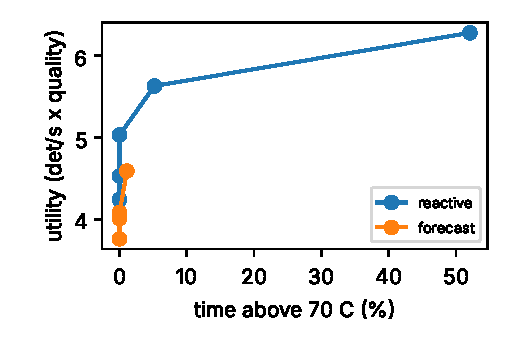
\includegraphics[width=\columnwidth]{figures/f_pareto.pdf}
\caption{Utility versus time above $70^\circ$C, cool-room scenario\SIM: reactive
thresholds shifted by $-12\ldots{+}4^\circ$C versus forecast target
$60\ldots76^\circ$C ($H{=}120$\,s).}\label{fig:pareto}
\end{figure}
\begin{table}[t]
\centering\small
\caption{Simulator fidelity: fitted plant versus device (E7).}\label{tab:fidelity}
\begin{tabular}{lrrr}
\toprule
Arm & Metric & Device & Simulator \\
\midrule
Static nominal & $>$70\,\textdegree C \% & \TBD{} & \TBD{} \\
Static nominal & Throttled \% & \TBD{} & \TBD{} \\
Static nominal & Max T & \TBD{} & \TBD{} \\
SHADE & $>$70\,\textdegree C \% & \TBD{} & \TBD{} \\
SHADE & Throttled \% & \TBD{} & \TBD{} \\
SHADE & Max T & \TBD{} & \TBD{} \\
\bottomrule
\end{tabular}
\end{table}

\textbf{Threats\SIM.} One plant family; an estimator that is well-specified for the
base plant; invented profiles. \TBD{After E7: report whether simulated and
measured time-above-$70^\circ$C agree for the same policy, and re-run the
ablation with the fitted plant.}
